
\documentclass[mathserif, aspectratio=169]{beamer}

\usepackage{psfrag,graphicx}
\usepackage{amsmath}
\usepackage[absolute,overlay]{textpos}

\usepackage{braket}
\graphicspath{{figs/}}

\usetheme{Boadilla}
\makeatother
\setbeamertemplate{footline}[frame number]

\usepackage{graphicx}
\usepackage{caption}
\usepackage{subcaption}
\captionsetup{compatibility=false}
\usepackage{amsmath} 
\usepackage{amssymb} 
\usepackage{amsthm}  
\usepackage{bm}
\usepackage{lipsum}
\usepackage[linesnumbered, ruled]{algorithm2e}
\usepackage{color}
\newtheorem{assumption}{Assumptions}
\newtheorem{prop}{Proposition}
\newtheorem{defn}{Definition}
\newtheorem{thm}{Theorem}
\newtheorem{lem}{Lemma}
\newtheorem{cor}{Corollary}
\newtheorem{sol}{Decentralized Solution}
\newtheorem{thresh}{$\epsilon$-thresholding}
\definecolor{light-gray}{gray}{0.8}
\usepackage{textcomp}

\newcommand{\backupbegin}{
   \newcounter{finalframe}
   \setcounter{finalframe}{\value{framenumber}}
}
\newcommand{\backupend}{
   \setcounter{framenumber}{\value{finalframe}}
}
\newcommand{\norm}[1]{\left\lVert #1 \right\rVert}

\makeatletter
\setbeamertemplate{navigation symbols}{}

\title[Lecture 28] 
{Data, Environment and Society: \\{Lecture 28: Neural Networks}}



\author[ER190C: Data, Environment and Society] 
{Instructor: Duncan Callaway\\
GSI: Seigi Karasaki} 

%\logo{
%\includegraphics[width=1.5cm,height=1.5cm,keepaspectratio]{uvic_logo_h.jpg}
%}
\vspace{-20mm}
\institute[UC Berkeley] % (optional, but mostly needed)
 {\small{ \bf December 3, 2018}}

\date[December 3, 2018]

\begin{document}

\frame{
	\titlepage
}


\begin{frame}{Announcements}
	\begin{itemize}
		\item Please do your course evaluations, \url{https://course-evaluations.berkeley.edu}
		\item Projects due on bcourses Dec 11 6pm.
		\item Please contact me or Seigi by email with questions.  
	\end{itemize}
\end{frame}


\begin{frame}{Today's outline}
	\begin{itemize}
		\item Neural networks (NN) -- very brief introduction
		\item A prediction application for NN: predicting poverty
		\item Course wrap-up
		\begin{itemize}
			\item What I hope you've learned
			\item Next steps?
		\end{itemize}
	\end{itemize}
\end{frame}


\begin{frame}
	\frametitle{Neural networks: Origins}
	\begin{columns}[c]
		\column{0.5\textwidth}
			\begin{itemize}
				\item The name is due to analogy with brains
				\begin{itemize}
					\item But the original purpose was not to reproduce cognition
				\end{itemize}
				\item First developed in 1943
				\item Little research activity $\sim$1960-1990's.  
				\item Computing advances made ``deep'' NN possible in the last 20 years
			\end{itemize}
		\column{0.5\textwidth}
			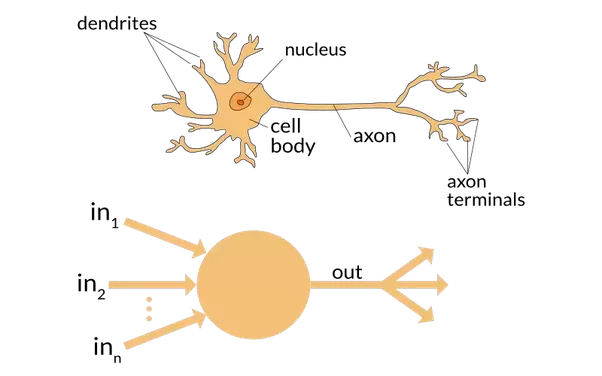
\includegraphics[width=\textwidth]{nn_v_ann}
	\end{columns}
\end{frame}


\begin{frame}{Mathematics for a single ``neuron''}   
    \begin{columns}
    	\column{0.5\textwidth}
    		In words, each neuron...
    		\begin{itemize}
    			\item Takes a vector of values as inputs
    			\item Creates a scalar from a linear combination of the vector entries
    			\item Passes the resulting scalar through an ``activation function''
    			\item Outputs a single value from that activation function
    		\end{itemize}
    	\column{0.5\textwidth}
	    	
    \end{columns}
\end{frame}


\begin{frame}[t]\frametitle{What's $f$, the activation function?}
    \begin{enumerate}
    	\item sigmoid
    	\vspace{15mm}
    	\item $\tanh$
    	\vspace{15mm}
    	\item rectified linear
    \end{enumerate}
\end{frame}

\begin{frame}[t]\frametitle{Neural network: just gang the neurons together}
    
\end{frame}


\begin{frame}[t]\frametitle{Mathematical merging of neurons}
    Convention:
    \begin{itemize}
    	\item $\alpha_{ij}^{(l)} \rightarrow$ weight from node $j$ in layer\\ $l$ to node $i$ in $l+1$ layer.
    	\item $a_{i}^{(l)} \rightarrow$ output of node $i$ in layer $l$.
    	\item $z_i^{(l)} \rightarrow$ input into node $i$ in layer $l$.
    \end{itemize}

    \begin{columns}
    	\column{0.5\textwidth}
    	    \begin{align*}
		     	a_1^{(2)} &= \\
		     	a_1^{(3)} &= \\
		    \end{align*}
	    \column{0.5\textwidth}
    \end{columns}
    
    Question: What are the parameters of a neural network model?
\end{frame}

\begin{frame}[t]\frametitle{Thinking about the features and target}
    Let's watch this video.  It uses graphics in a nice way to explain what NNs are doing. 
    \vspace{10mm}

    \url{https://www.youtube.com/watch?v=aircAruvnKk}

    \vspace{10mm}

    Start the video at 2:05.  We'll stop watching around 5:30.
\end{frame}


\begin{frame}[t]\frametitle{Fitting the model}
	Training data: $\{(x_1,y_1), (x_2,y_2), \hdots, (x_n,y_n)\}$

	\vspace{5mm}

	$x_k \in \mathbb{R}^p$ ($p$ features)\\
	$y_k \in \mathbb{R}^K$ ($k$ outputs)

	Objective function: 

\end{frame}

\begin{frame}[t]\frametitle{Quick notes on objective function}
    
	\begin{itemize}
	 	\item Form is amenable to classification, just one-hot encode the output and use classification error rate as your objective
	 	\item For regression, be sure to scale the output variables to lie in the range of the activation function.  
	\end{itemize} 

\end{frame}

\begin{frame}[t]\frametitle{Fitting the model, ctd}
	\begin{description}
		\item[Step 1] Initalize parameters
		\item[Step 2] Identify optimal parameters by gradient search.
	\end{description}
\end{frame}

\begin{frame}[t]\frametitle{Tensorflow playground}
    On \href{http://playground.tensorflow.org}{\textbf{this website}} you'll find a cool interactive tool that allows you to play with NN for classification.

    \vspace{5mm}

    \begin{enumerate}
    	\item What are the hyperparameters of the model?  Can you explain what each one does?
    	\item Try fitting the ``exclusive or'' (choose on top left) data set.
    	\item Also try fitting the ``Spiral'' data set.  
    	\item Possible spiral solution:
    	\begin{enumerate}
    		\item<2-> Two hidden layers
    		\item<2-> Sigmoid activation
    		\item<2-> Include all but $X_1X_2$ features.
    		\item<2-> L1 regularization
    	\end{enumerate}
    	\item<3-> You got close by trial and errror.  What's another way?
    	\begin{itemize}
    		\item<4-> Grid search; randomized search and cross validation! 
    		\item<4-> There are other more advanced ways...
    		\item<4-> But everything is computationally intense.  
    	\end{itemize}
    \end{enumerate}
\end{frame}

\begin{frame}{Example resource allocation with NN}
\begin{figure}
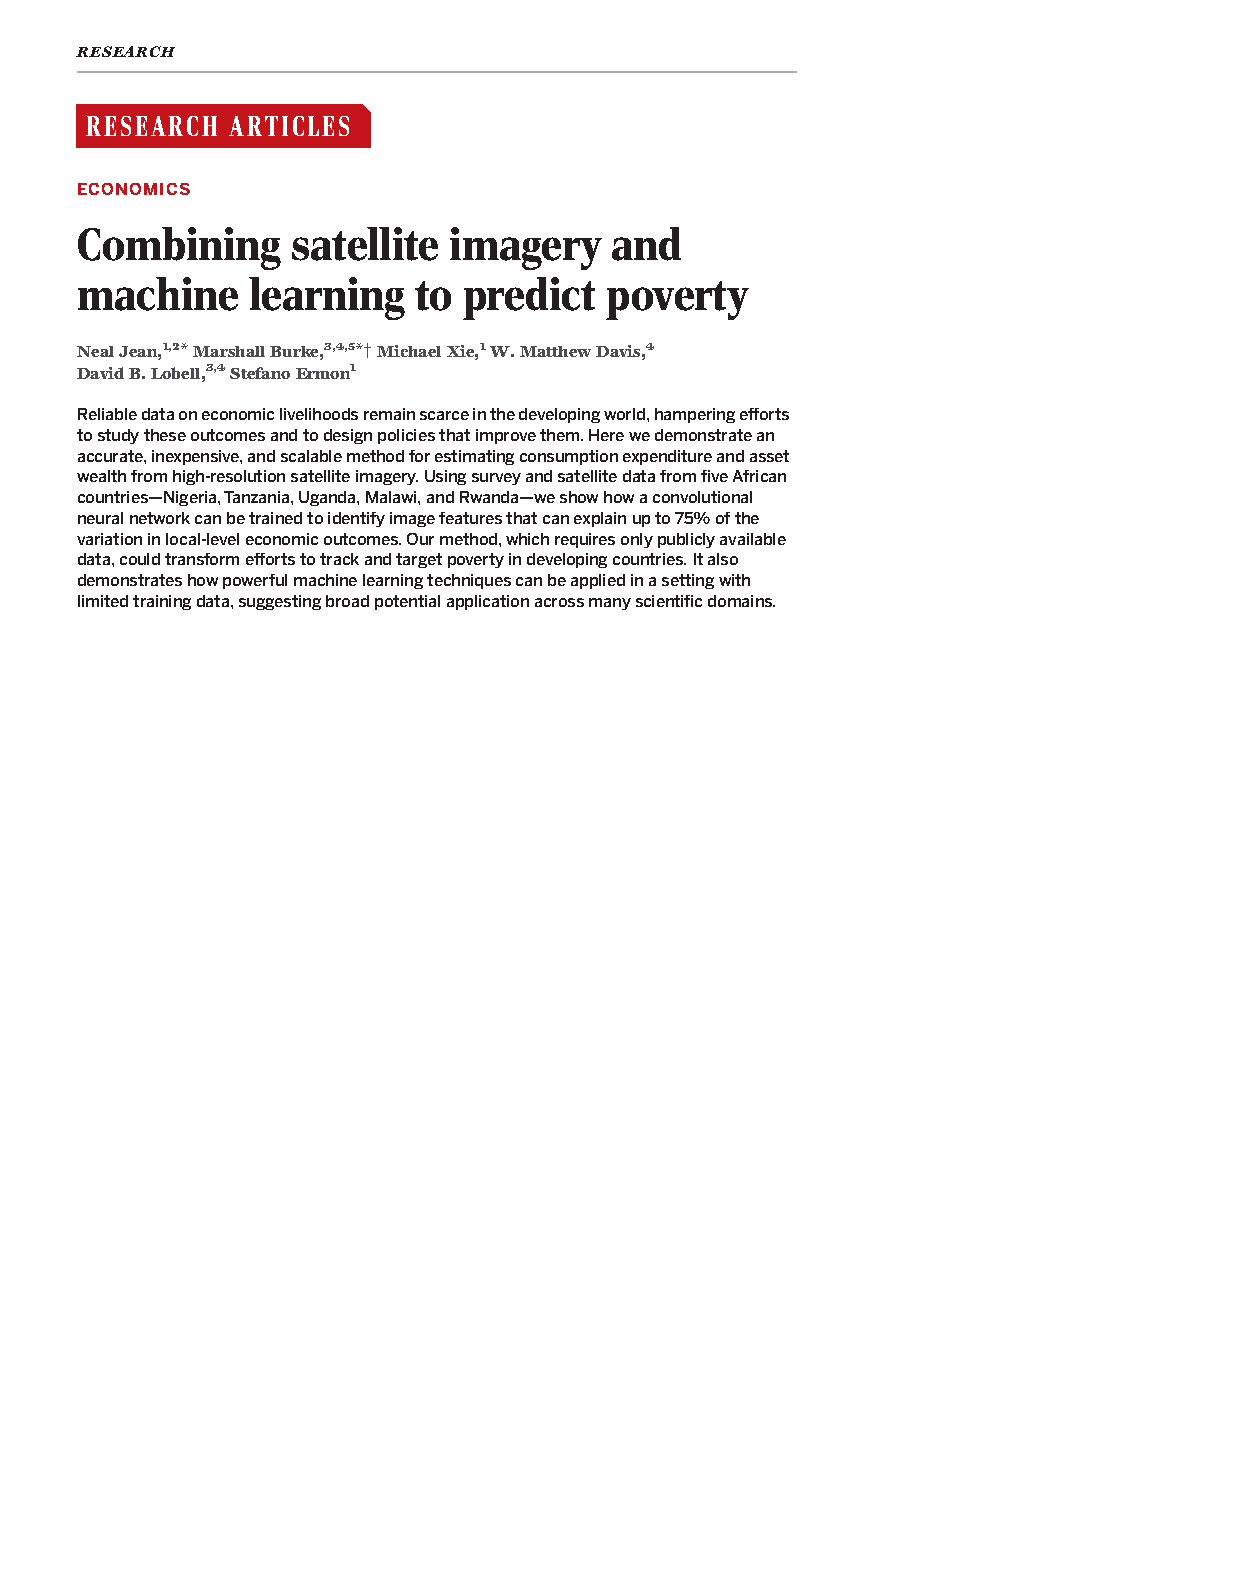
\includegraphics[width=0.7\textwidth]{jean_header}
\caption*{}
\end{figure}
\end{frame}

\begin{frame}{The challenge}

\begin{itemize}
\item International aid agencies want information on where to spend effort
\item Knowing where the poorest people are can inform these decisions
\item But surveying a country's population is expensive, and most survey results are not in the public domain.  
\begin{itemize}
\item About 25\% of African countries did not run any surveys between 2000-2010 from which poverty measures could be computed. 
\end{itemize}
\item Question: can one train a model that uses remote sensing data to predict poverty?
\end{itemize}

\end{frame}

\begin{frame}{Night lights}

	\begin{itemize}
		\item Some folks have used night satellite imagery to estimate spatial distributions of wealth
			\begin{itemize}
				\item Basic idea: satellites can see lighting activity at night; People with more money use more night lighting.  
			\end{itemize}
		\item These methods are not accurate at extreme poverty income levels ($<\$1.90$ per person per day)
		\item There is little data on extreme poverty (see previous slide) so there isn't a large data set to train models with.
	\end{itemize}
	\begin{center}
		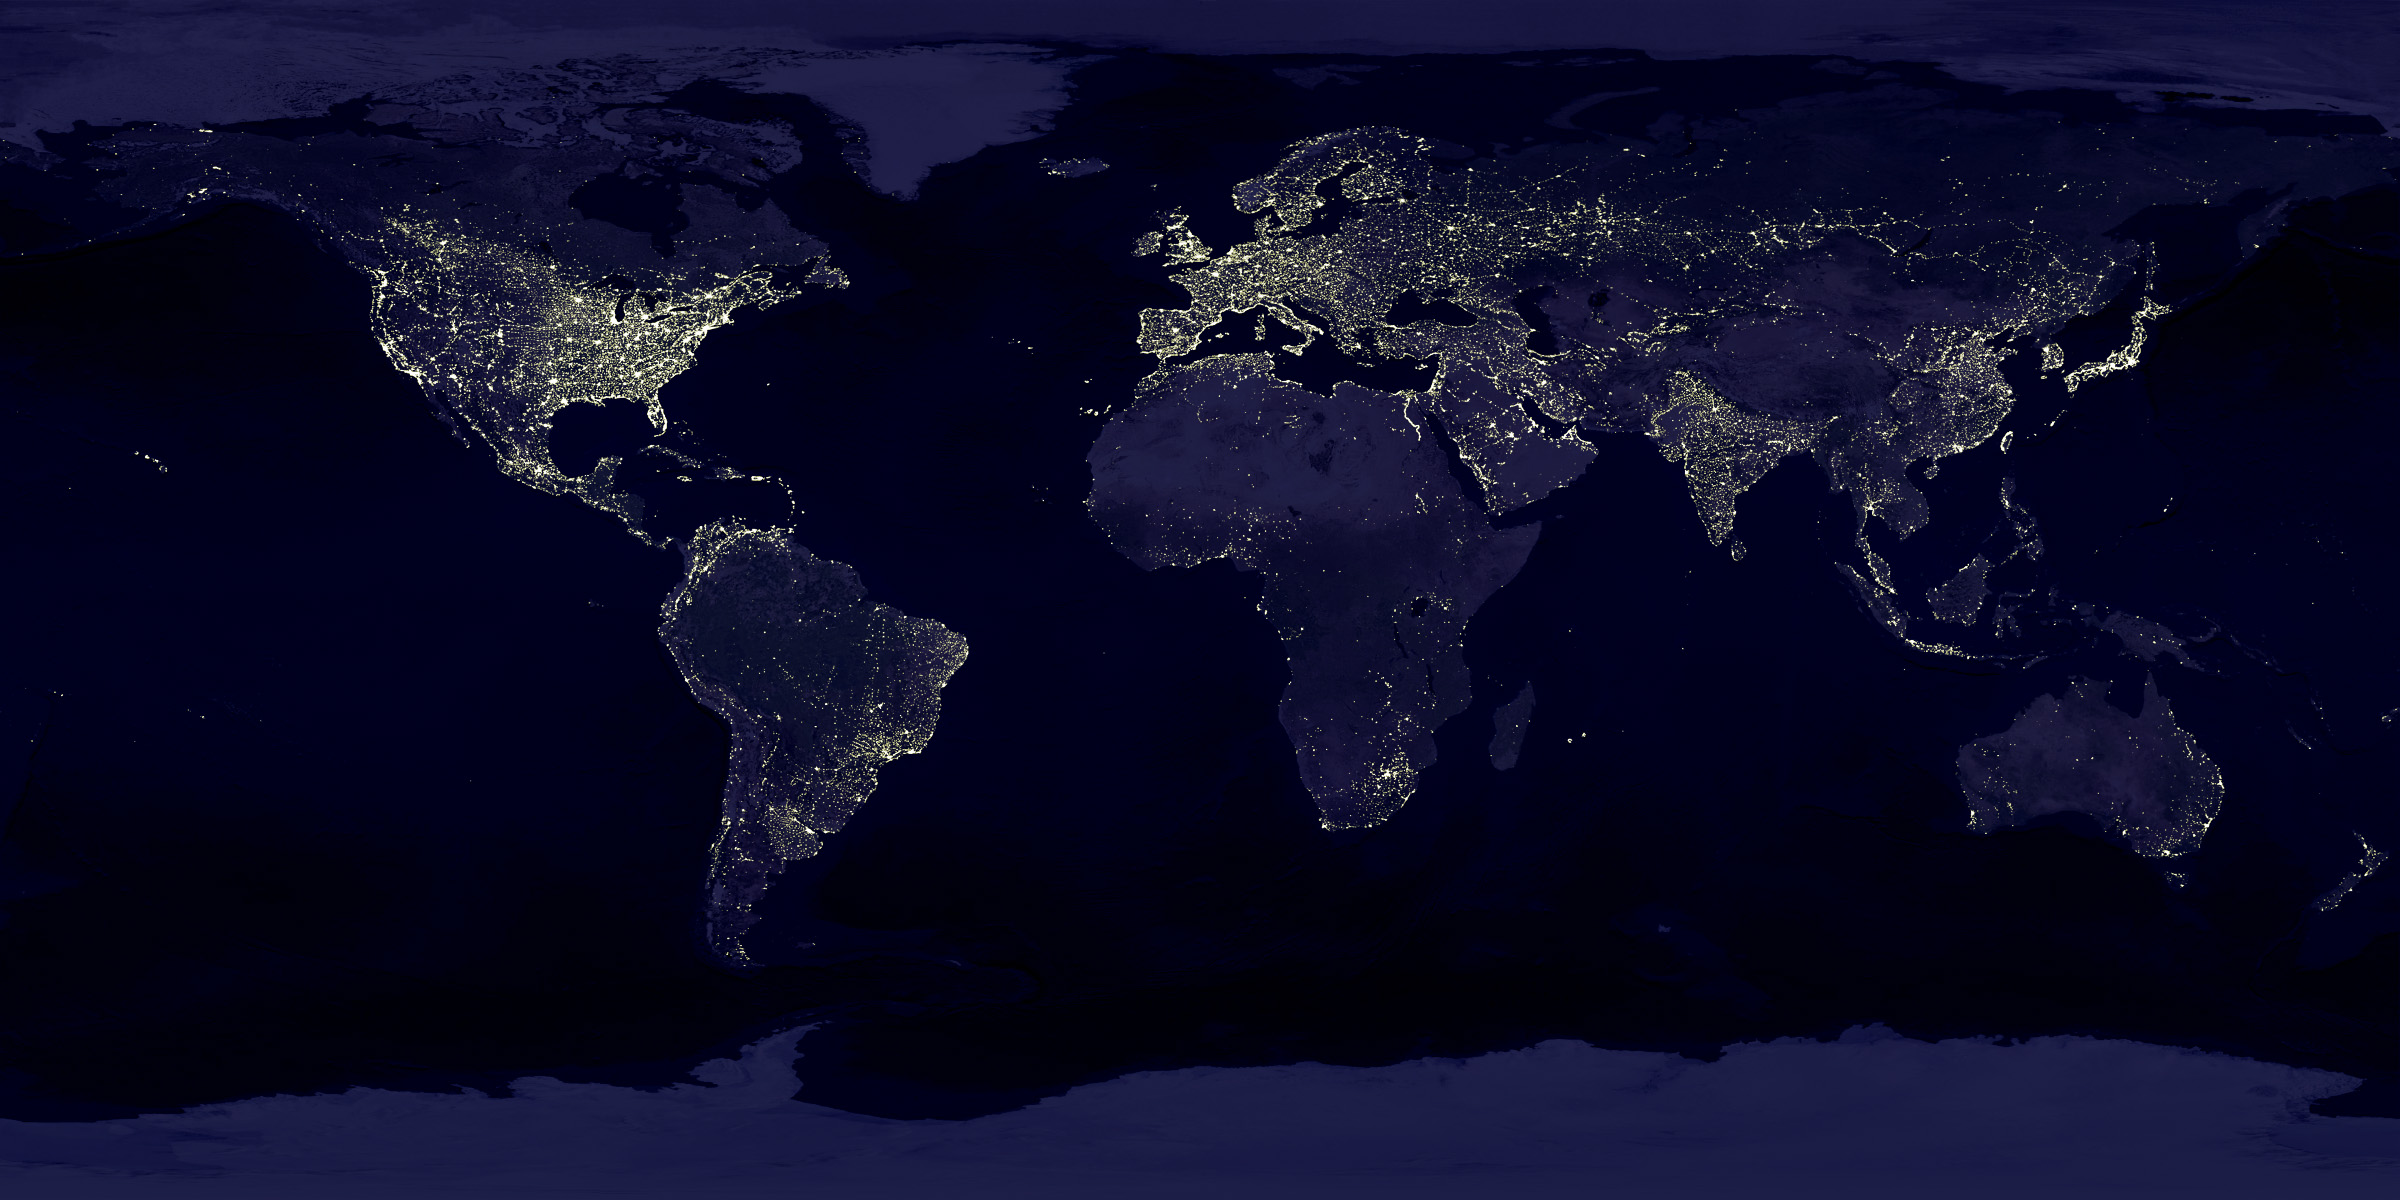
\includegraphics[width=0.6\textwidth]{earth_lights_lrg}
	\end{center}
\end{frame}

\begin{frame}{Jean \textit{et al's} idea}
\begin{enumerate}
\item Use \textit{daytime }satellite imagery, not night time
\begin{itemize}
\item Landcover type and structures, for example, ought to help to predict poverty.
\end{itemize}
\item Deal with the data paucity problem via ``transfer learning''
\begin{itemize}
\item The idea here is pretty simple: train a neural net on a well known set of images (ImageNet -- labelled data from 1,000 categories, e.g. ``boneshaker'', ``crutch'', ``miniature schnauzer'')

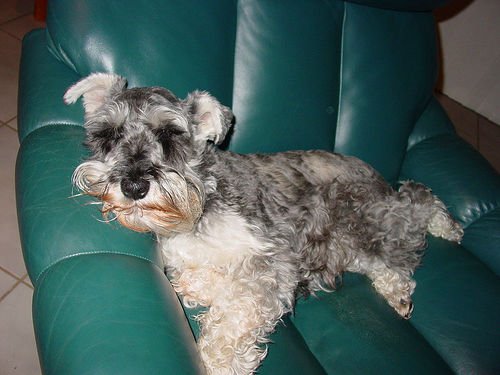
\includegraphics[height=0.3\textheight]{schnauzer} \;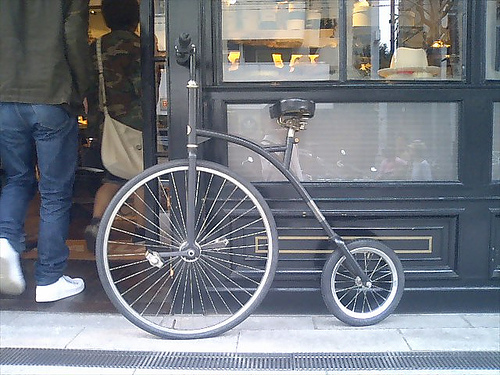
\includegraphics[height=0.3\textheight]{boneshaker}\;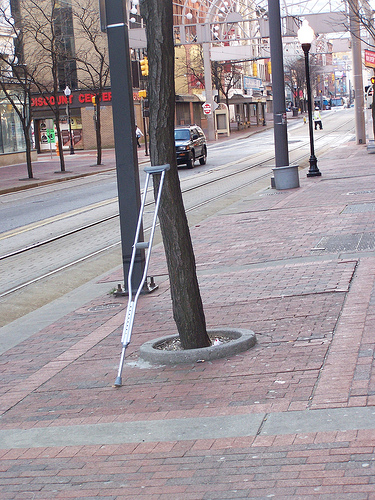
\includegraphics[height=0.3\textheight]{crutch.jpg}

\item the model learns to identify low- level image features such as edges and corners that are common to many vision tasks
\end{itemize}
\end{enumerate}
\end{frame}

\begin{frame}{A bit more on Jean \textit{et al's} transfer learning}
\begin{enumerate}
 \setcounter{enumi}{2}
\item ImageNet-trained model then ``fine tuned'' to use daytime satellite imagery inputs to predict the nighttime light intensities outputs.
\begin{itemize}
\item In doing this Jean\textit{ et al} are falling back on the idea of using night lights (or a prediction of night lights) to measure income and wealth
\item It's desirable to use night lights because it's a globally available data set and is a better proxy for economic activity than the daytime images would be.
\end{itemize}
\item Then build a ridge regression model:
\begin{itemize}
	\item Target: mean cluster-level values from \textit{survey} data (where available) 
	\begin{itemize}
		\item Clusters are geographic areas approximately the size of a village.
	\end{itemize}
	\item Features: the corresponding image features extracted from daytime imagery by the NN 
\end{itemize}
\end{enumerate}
\end{frame}

\begin{frame}{Basic summary of process}

\begin{itemize}
\item Old: night lights $\rightarrow $ predict wealth and income
\item New: daytime imagery $\rightarrow$ predict night lights $\rightarrow$ predict wealth and income.
\end{itemize}

\end{frame}

\begin{frame}{Wait -- I thought night lights were a lousy proxy for economic activity at low income levels?}

\begin{itemize}
\item Jean \textit{et al} address (or try to address) this head on.  
\item Their claim is that because they're using a linear model (ridge regression) to map day time imagery to  night lights, the model is going to be driven by light-economic relationships at higher income levels.  
\begin{itemize}
 \item If they're lucky, the lower income relationship between \textit{estimated} night lights and economic activity will be decent.
 \end{itemize} 
\end{itemize}
\end{frame}

\begin{frame}
	\frametitle{Results}
	\begin{columns}[c]
		\column{0.5\textwidth}
			\includegraphics[width=1\textwidth]{jean_fig3}
		\column{0.5\textwidth}
			\includegraphics[width=1.1\textwidth]{jean_figS3}
	\end{columns}
\end{frame}


\begin{frame}{A side note on using models trained on one data set to interpret another}
	Image classification:
	\begin{itemize}
		\item Each layer of NN extracts higher and higher-level features of the image
		\item The final layer makes a decision on what the image shows. 
		\item Example: 
		\begin{itemize}
			\item First layer might look for edges or corners. 
			\item Intermediate layers interpret basic features to identify components (wheel, cliff...)
			\item Final layers assemble those into complete interpretations (bicycle, mountain range...)
		\end{itemize}
		\item Google researchers played around with this:
		\begin{itemize}
			\item Starting with an NN trained on ImageNet
			\item Have the NN interpret new images
			\item Look at intermediate layers of the interpretation
		\end{itemize}
	\end{itemize}

	More information \href{https://ai.googleblog.com/2015/06/inceptionism-going-deeper-into-neural.html}{\textbf{here}}.

\end{frame}

\begin{frame}{Example: Low layer interpretation}
Here we see accentuation of strokes and colors.
\begin{figure}
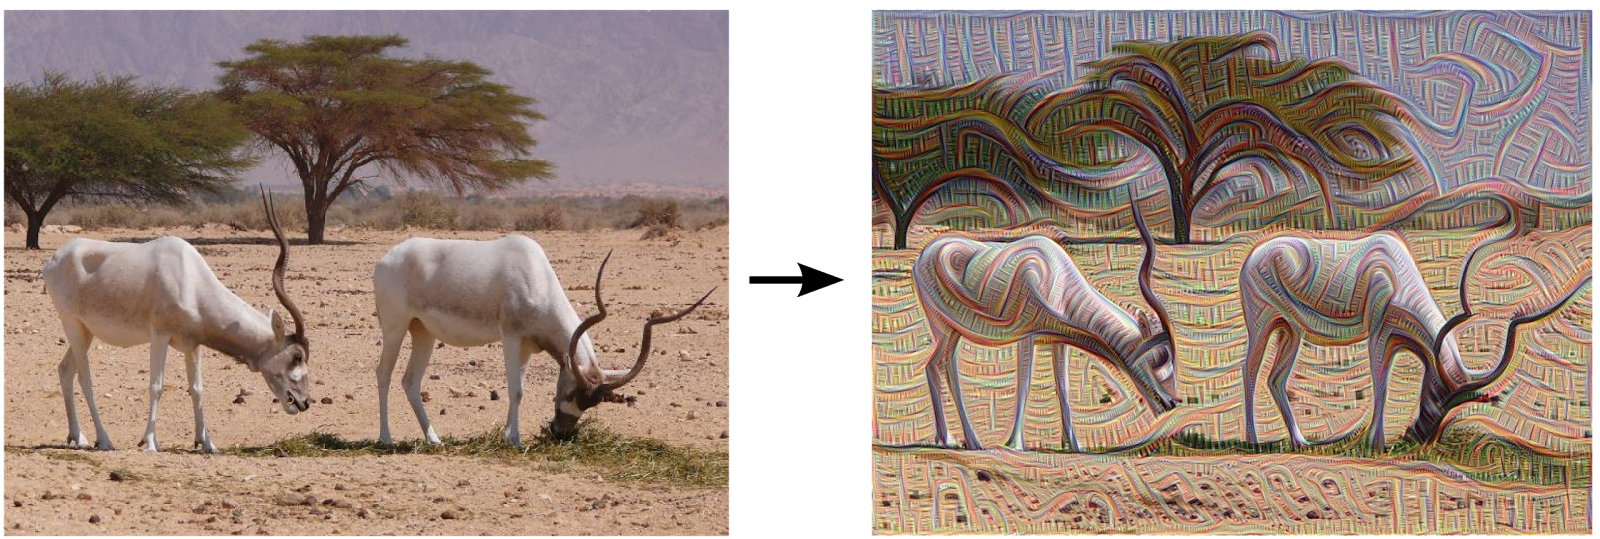
\includegraphics[width=\textwidth]{ibis_google}
\caption*{}
\end{figure}
\end{frame}

\begin{frame}{Example: High layer interpretation}
Here we see accentuation of specific kinds of features
\begin{figure}
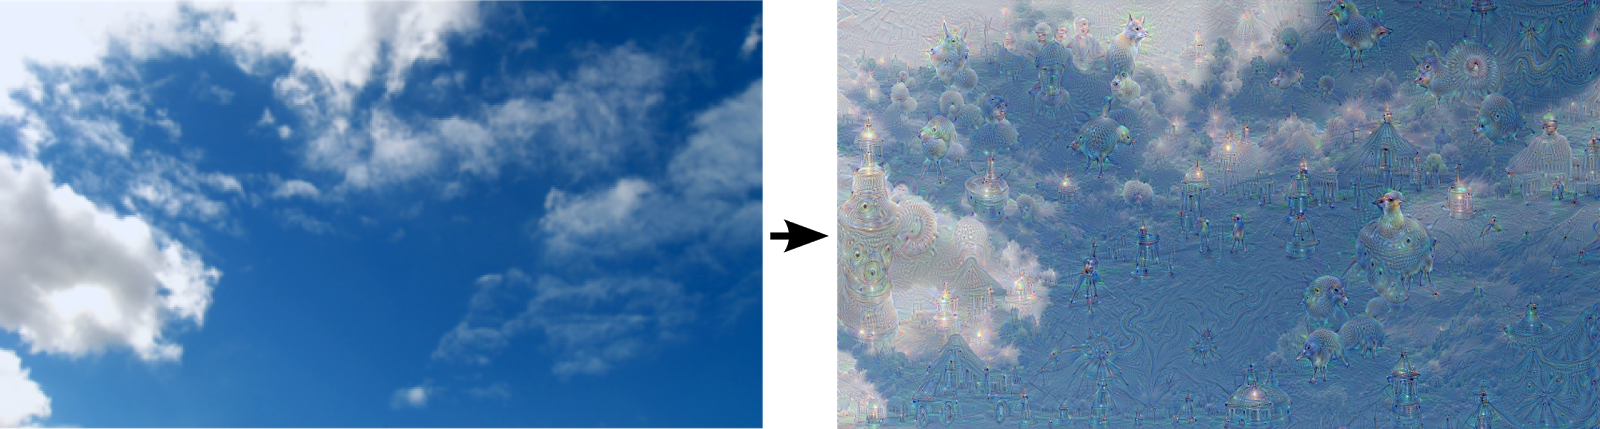
\includegraphics[width=\textwidth]{skyarrow_google}
\caption*{}
\end{figure}
\end{frame}

\begin{frame}{A zoom in on the cloud images}
\begin{figure}
\includegraphics[width=\textwidth]{funny-animals_google}
\caption*{}
\end{figure}

\vspace{-10mm}
\pause
Are these the dreams of neural networks?
\begin{itemize}
	\item Reporters that covered the research liked to spin it that way
	\item I tend to think of this more pragmatically -- these are just complex mathematical interpretations of images.
	\item BUT: I do think the images are beautiful and related to the way humans play with images
	\item This certainly pushes computing in the direction of art and spirituality, which I find scary and inspiring
\end{itemize}
\end{frame}

\begin{frame}[t]\frametitle{}
	\textbf{Course wrapup: What do I hope you've learned?}
\end{frame}

\begin{frame}
	\frametitle{Python}
	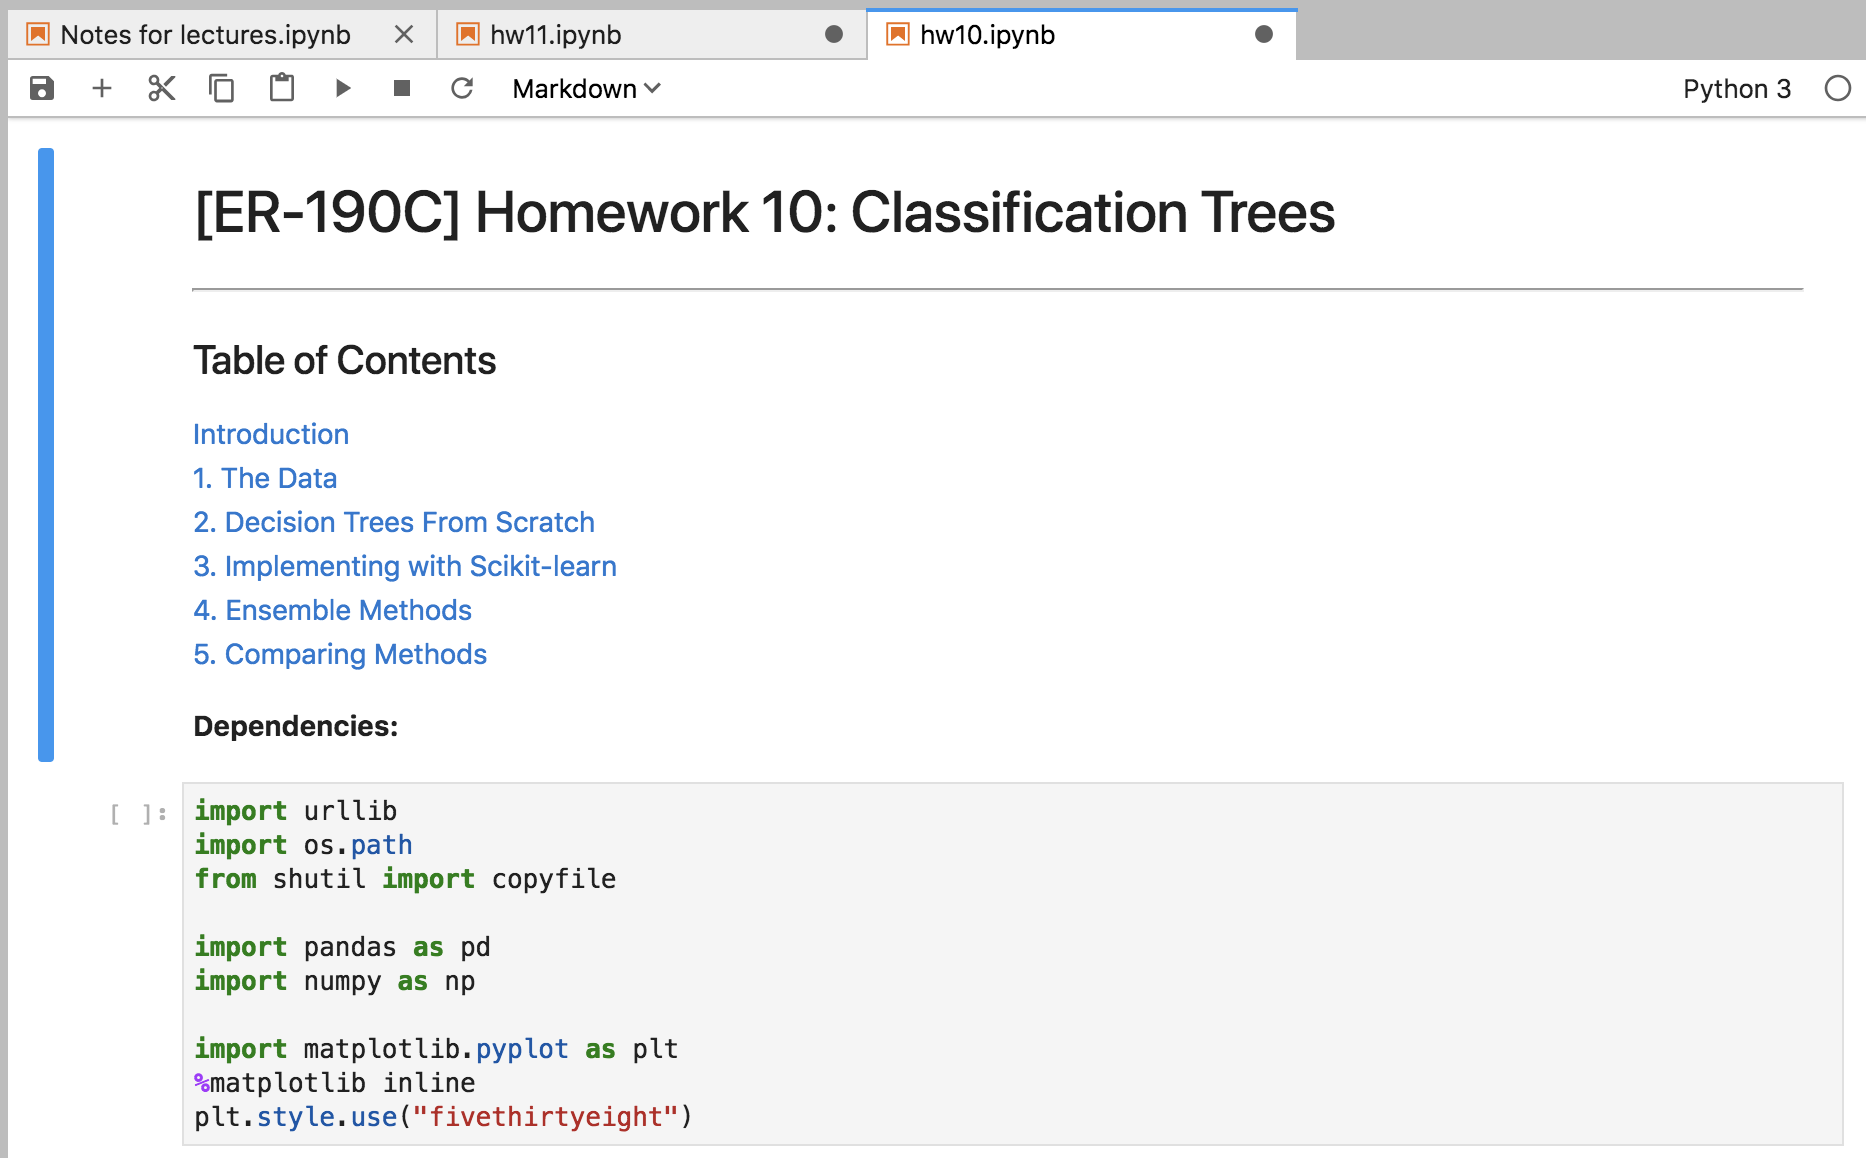
\includegraphics[height=\textheight]{python}
\end{frame}

\begin{frame}
	\frametitle{Visualization}
	\begin{center}
		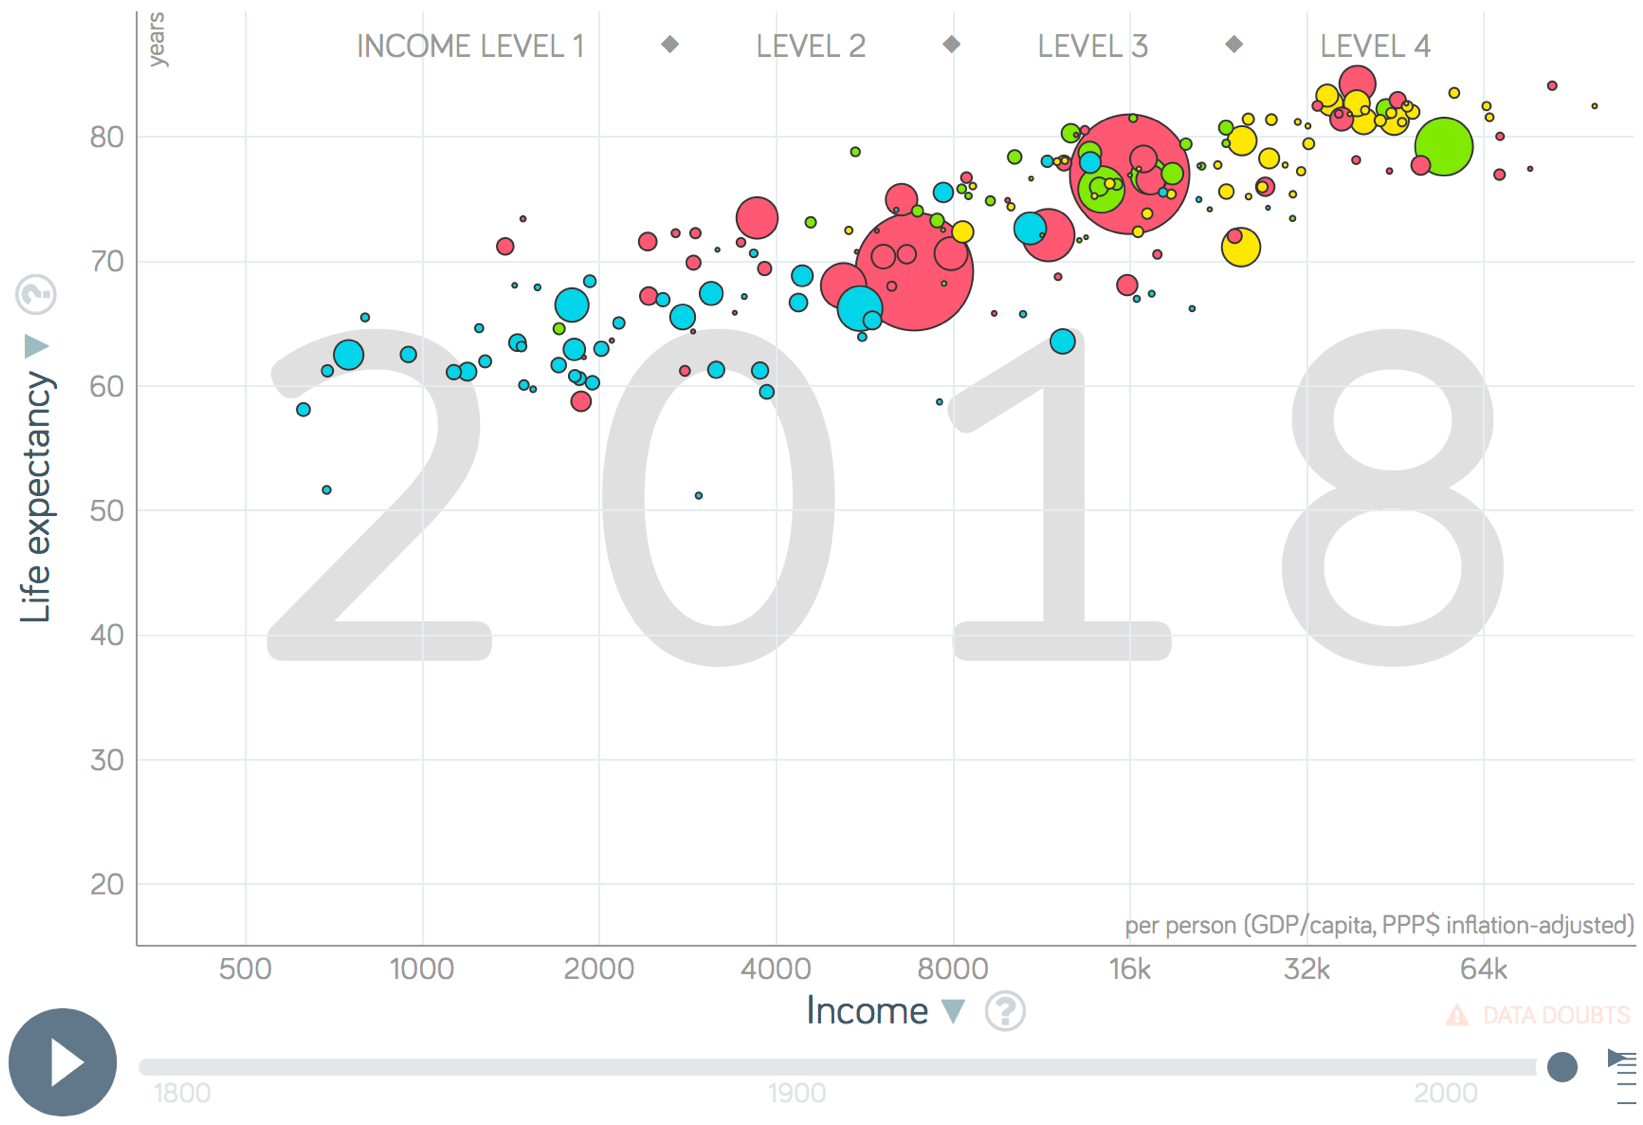
\includegraphics[height=0.9\textheight]{pop-income}
	\end{center}
\end{frame}

\begin{frame}
	\frametitle{Resampling}
	\begin{center}
		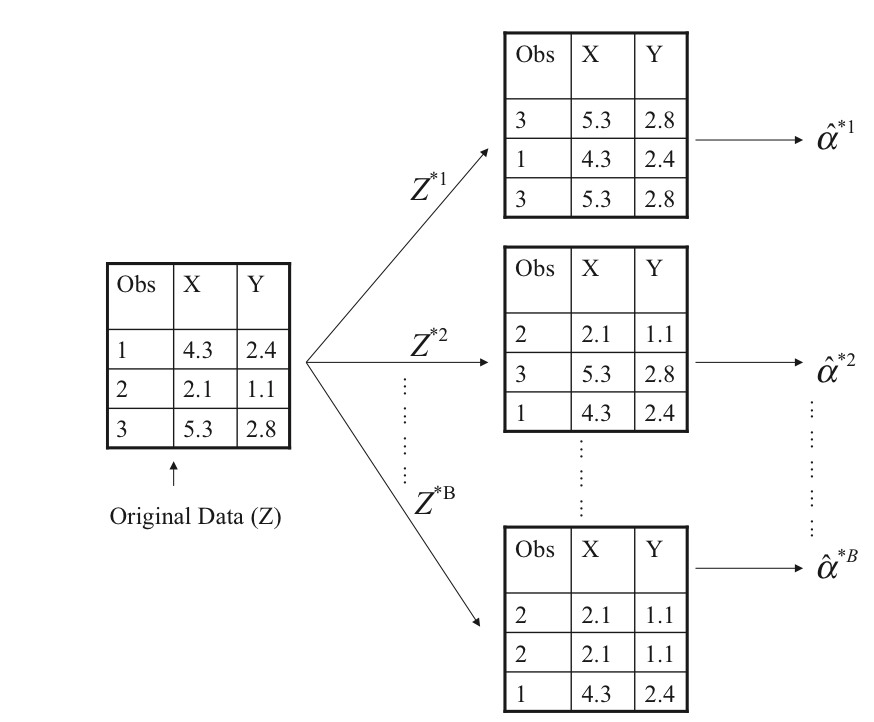
\includegraphics[height=0.65\textheight]{bootstrap}
		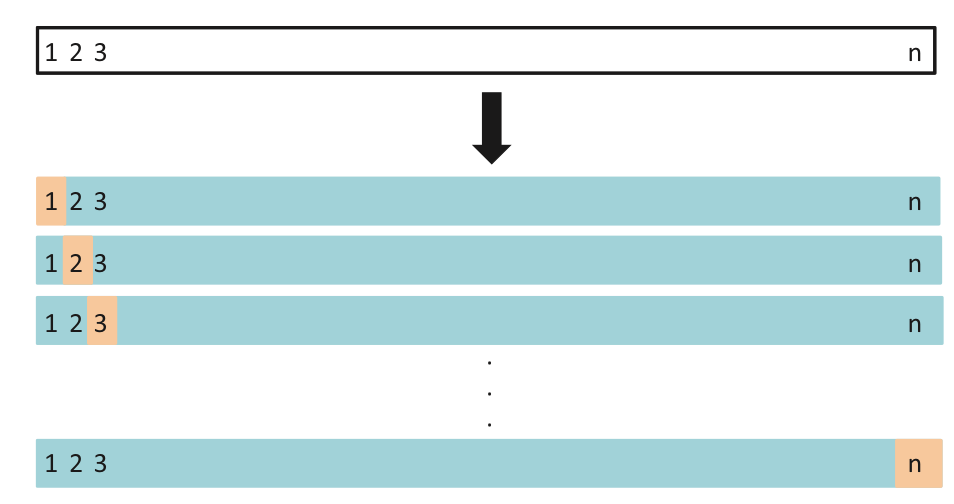
\includegraphics[height=0.5\textheight]{loocv}
	\end{center}
\end{frame}

\begin{frame}
	\frametitle{Model identification}
	\begin{itemize}
		\item Parameters fit by loss minimization
		\begin{itemize}
			\item These determine the shape of the function you're fitting
		\end{itemize}
		\item Hyperparameters fit by iteration and cross validation
		\begin{itemize}
			\item These enable you to tune bias-variance tradeoff
		\end{itemize}
	\end{itemize}
\end{frame}


\begin{frame}{Zoom out: Train, (cross) validate and test}
	Using slightly different language, some definitions from from Brian Ripley, Pattern Recognition and Neural Networks, 1996, page 354:
	\vspace{5mm}
	\begin{itemize} 
		\item \textbf{Training set}: ``A set of examples used for learning, that is to fit the parameters of the classifier.''
		\begin{itemize}
			\item{For minimizing the loss function}
		\end{itemize}
		\item\textbf{ Validation set}: ``A set of examples used to tune the parameters of a classifier, for example to choose the number of hidden units in a neural network.''
		\begin{itemize}
			\item For choosing hyperparameters.
		\end{itemize}
		\item \textbf{Test set}: ``A set of examples used only to assess the performance of a fully-specified classifier.''
		\begin{itemize}
			\item For a final check -- no more model fitting allowed here!
		\end{itemize}
	\end{itemize}
	\vspace{5mm}
\end{frame}



\begin{frame}
	\frametitle{New tools for prediction: regression and classification}
	\begin{columns}[c]
		\column{0.7\textwidth}
			\begin{itemize}		
				\item Linear regression models: Ridge, Lasso, Elastic net
				\begin{align*}
					\min_\beta \sum_{i=1}^N \left(Y_i - X_i \beta \right)^2+\lambda \cdot R(\beta)
				\end{align*}
				\item Decision trees
				\item Support vector machines
			\end{itemize}
		\column{0.25\textwidth}
			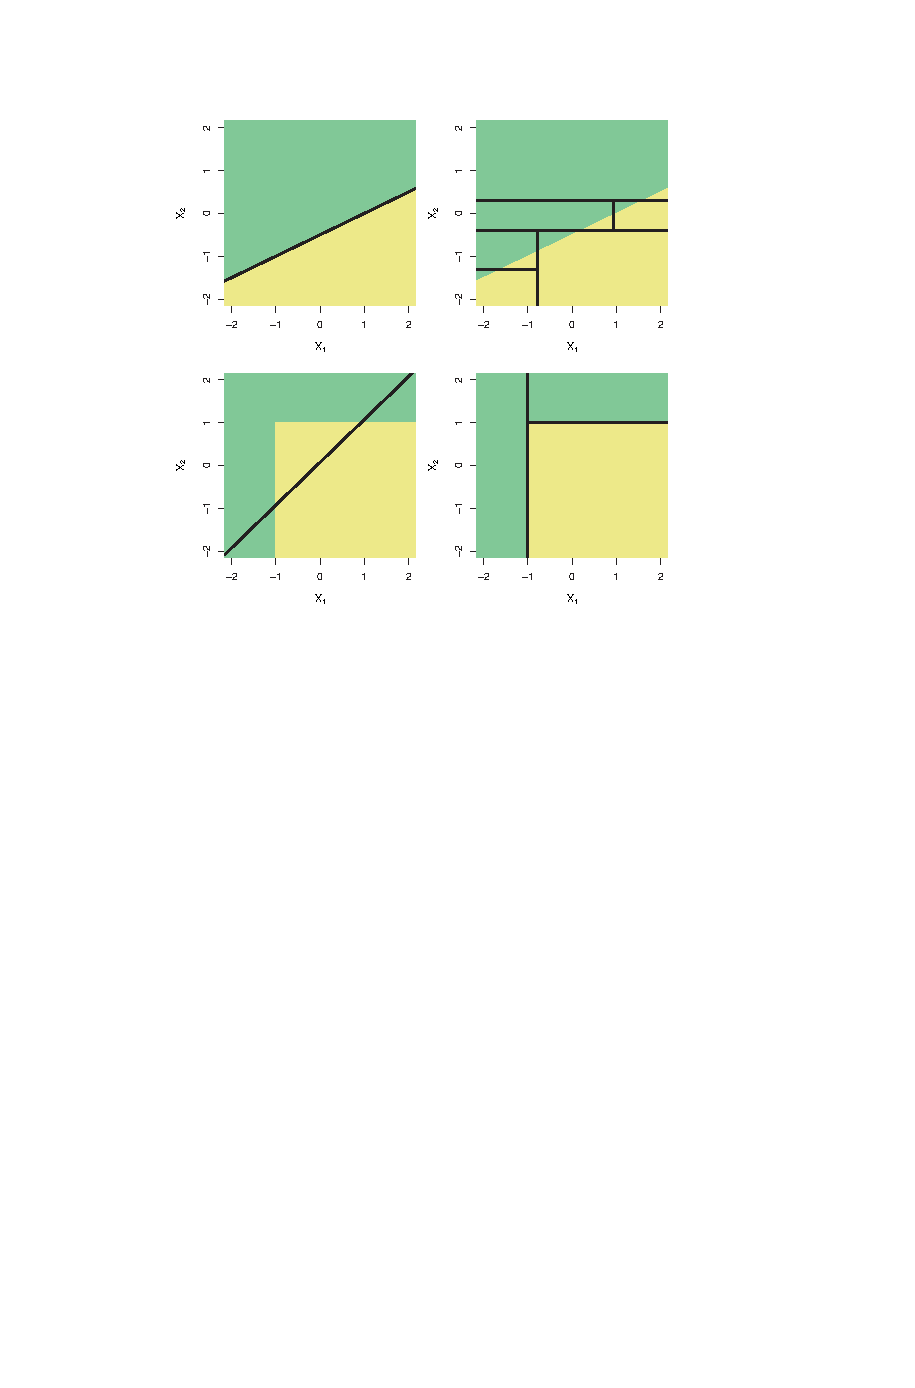
\includegraphics[width=\textwidth]{tree_vs_linear_for_classification}

			\includegraphics[width=\textwidth]{SVM_example}
	\end{columns}
\end{frame}

\begin{frame}
	\frametitle{Inference, prediction and resource allocation in environmental contexts}
	\begin{columns}[c]
		\column{0.3\textwidth}
			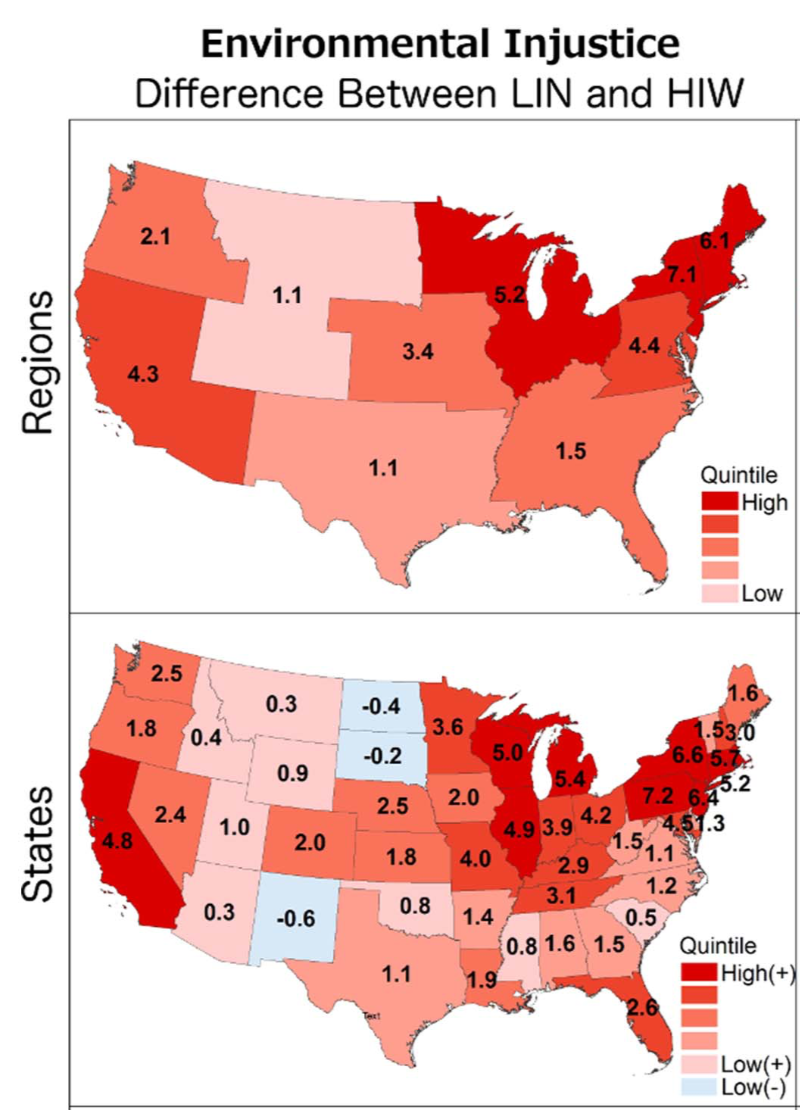
\includegraphics[width = \textwidth]{marshall_injustice}
		\column{0.7\textwidth}
			\begin{itemize}
				\item Prediction in space: what's happening in places where I have limited data?
				\begin{itemize}
					\item Example: What are the NO2 concentrations where we don't have monitoring equipment?
					\item Example: What are the land cover characteristics in a region?
				\end{itemize}
				\item Prediction across communities: What's happening in communities where I have limited information?  
				\begin{itemize}
					\item Example: What communities in California have clean water?
				\end{itemize}
				\item Prediction in time: What will happen next year, or tomorrow?  
				\begin{itemize}
					\item Example: will the air be clean tomorrow?
				\end{itemize}
			\end{itemize}
	\end{columns}
\end{frame}

\begin{frame}
	\frametitle{Next steps: What I hope for you}
	\begin{itemize}
		\item You've now got basic skills for data manipulation and modeling and working in Python
		\item You've also got experience developing research questions and defining resource allocation problems
		\item You should feel proud of these skills when you present yourself to potential research advisers and employers
		\begin{itemize}
			\item Environmental and Justice nonprofits and NGOs
			\item Government regulators
			\item Energy sector companies
		\end{itemize}
		...all these folks are looking for the skills you now have
		\item You're also ready to take more courses in the area: DS100, CS189, Stat 154.
		\item I also hope you'll keep in touch -- tell me how you use these skills!
	\end{itemize}
\end{frame}


\end{document}
